\section{Introduction}

Recent advances in small Unmanned Aircraft Systems (UAS) perception systems are beginning to enable safe three-dimensional small UAS navigation through complex uncertain environments for applications such as aerial photography, infrastructure inspection, search and rescue, and package delivery. Urban UAS operations will necessarily occur above buildings and over people. A safe urgent landing capability is a necessity, but no terrain-based or prepared vertiport landing option \cite{patterson_timely_2014, atkins_emergency_2006, di_donato_evaluating_2017} may be available.  In densely-populated urban regions, building rooftops can offer nearby safe landing zones for small UAS \cite{desaraju_vision-based_2015}. Urban roofs often have flat-like characteristics and are usually free from human presence \cite{castagno_roof_2018}. However, landing on urban buildings provides unique challenges such as avoiding auxiliary structures hosted on each rooftop.  A database of flat rooftops, their topologies, and optimal touchdown points can be computed and stored a priori from data such as satellite imagery and airborne survey point clouds \cite{castagno_map-based_2021}. However, the UAS must also confirm during approach that the rooftop landing zone is clear and replan as needed. 

\begin{figure}[!ht]
    \centering
    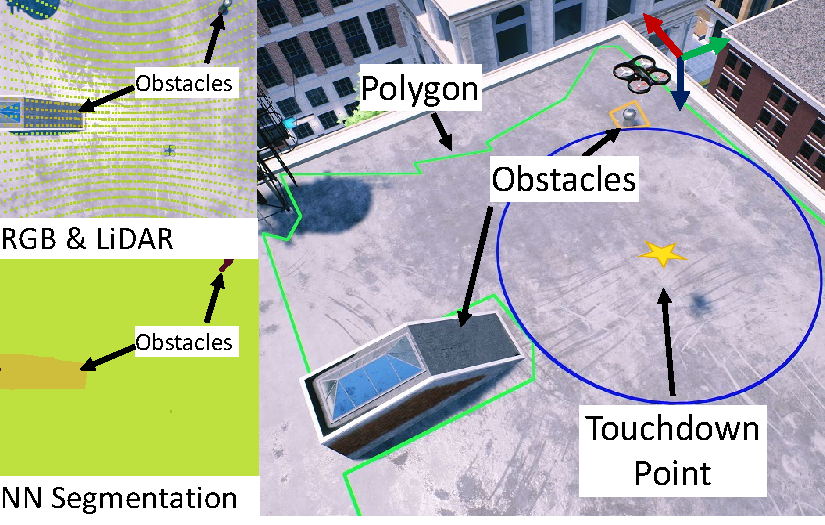
\includegraphics[width=0.75\columnwidth]{chapter_6_landingsim/figs/main_photo.pdf}
    \caption[Overview of Semantic Polylidar3D for real-time landing site selection]{Overview of Semantic Polylidar3D for landing site selection. Camera RGB (red-green-blue) images are transformed into a segmented image through a neural network. LiDAR point cloud data is projected into the segmented image for classification. Flat surfaces are extracted with Polylidar3D \cite{castagno_polylidar3d_2020} from the \textit{classified} point cloud distinguishing Semantic Polylidar3D as shown in the right image indicating a green candidate landing site polygon with orange interior ``obstacle cutouts''. The blue circle represents the largest flat, obstacle-free landing site.}
    \label{fig:ls_overview}
\end{figure}

This chapter proposes Semantic Polylidar3D, a suite of computational geometry (Polylidar3D \cite{castagno_polylidar3d_2020}) and deep neural network (semantic segmentation \cite{howard_mobilenets_2017, ronneberger_u-net_2015}) algorithms to identify and select safe rooftop landing zones in real time using a combination of LiDAR and camera sensors.  A high-fidelity simulated city is constructed in the Unreal game engine \cite{unrealengine} with particular attention given to creating a statistically-accurate representation of rooftop obstacles that create obstructions to safe landing, e.g., water towers, vents, air conditioning units, rooftop building access doors.    AirSim \cite{shah_airsim_2018}, a robotic vehicle simulator plugin for Unreal, generates onboard small UAS video and LiDAR data feeds as the small UAS navigates through the simulated Unreal environment.  Semantic Polylidar3D fuses \ac{sUAS} image and LiDAR data to compute the optimal obstacle-free touchdown circle on a rooftop within UAS sensor field of view. Figure \ref{fig:ls_overview} provides a graphical overview of processing steps. A LiDAR point cloud is classified by projecting data into a semantic image generated by a neural network. The classified point cloud is then rapidly converted into a polygon representing clear landing area accounting for both geometric and semantic information. Key contributions include:

\begin{itemize}
  \item Construction of a high-fidelity visual city model from real world data of the rooftops in midtown Manhattan, New York.
  \item A hybrid algorithm for planar extraction accounting for semantic information using computational geometry and deep learning.
  \item A novel landing site search and selection process for finding optimal touch down sites on rooftops in a processing pipeline viable for real-time deployment. 
  \item A comparative study of state-of-the-art semantic segmentation models to show their classification accuracy as well as time complexity.
%   \item Hardware In the Loop (HIL) results of our landing site selection algorithm on desktop and embedded (Jetson TX2) systems with real time performance comparison.
% and contingency planning
\end{itemize}
%  rooftop and obstacle identifying 

% Hard-coded numbers for speed of writing - Ella   (feel free to put in proper refs if you want the tex code to assure consistent numbers)
Below, a summary of related work (Section 2) is followed by a problem statement in Section 3.  Section 4 describes our landing site selection procedure using Semantic Polylidar 3D.  The urban rooftop simulation environment is presented in Section 5, and results are presented for semantic segmentation (Section 6) and the integrated Semantic Polylidar3D pipeline (Section 7).  The chapter concludes with a discussion (Section 8) followed by a brief conclusion (Section 9).